\documentclass[../../../main]{subfiles}

\begin{document}

% subsection %%%%%%%%%%%%%%%%%%%%%%%%%%%%%%%%%%%%%%%%%%%%%%%%%%%%%%%%%%%%%%%%%%%%%%%%%%%%%%%%%%%%%%%%%%%%%%%%%%%%
\subsection{Definition and Elementary Properties}

A {\it graph}\index{graph}, similar to a balanced incomplete block design, is simply an ordered pair $\Gamma = (V,E)$ where $V$ is a finite set of $v$ points, called {\it vertices}\index{vertex}, and where $E \subset \binom{V}{2}$, called the {\it edges}\index{edge}.\Cnote{simple-graph}

If $x,y \in V$ are distinct, and if $\{x,y\} \in E$, then we say that $x$ and $y$ are {\it adjacent}, and we write $x \sim y$. If there is a sequence of vertices $x = v_0, v_1, \dots, v_{n-1} = y$ such that $v_{i-1} \sim v_i$, for $i \in \{1,\dots,n-1\}$, then we say that $x$ and $y$ are {\it connected}\index{connected}. Connectedness is easily seen to be an equivalence relation of the vertex set $V$.

The {\it degree}\index{vertex!degree of} of vertex $x$ is defined as the number of vertices that are adjacent to $x$. If every vertex has the same degree, say, $k$, then we say that the graph is {\it regular}\index{graph!regular} with degree $k$.

The {\it complement}\index{graph!complement of} of a graph $\Gamma = (V,E)$ is given by $\bar\Gamma = (V,\binom{V}{2} \bb E)$.

\begin{ex}\label{petersen}\index{Petersen graph}
 The following is a graph on $10$ vertices called the {\it Petersen graph}, where the vertices are the nodes, and where the line segments represent adjacencies. One can see that each pair of distinct vertices are connected.
 \begin{defenum}
\item 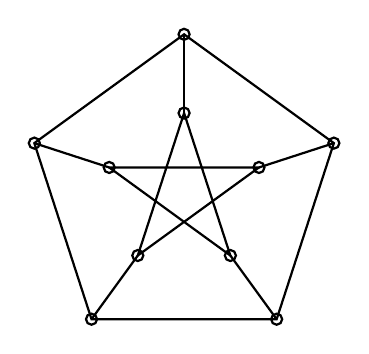
\begin{tikzpicture}[style=thick]
\draw (18:2cm) -- (90:2cm) -- (162:2cm) -- (234:2cm) --
(306:2cm) -- cycle;
\draw (18:1cm) -- (162:1cm) -- (306:1cm) -- (90:1cm) --
(234:1cm) -- cycle;
\foreach \x in {18,90,162,234,306}{
\draw (\x:1cm) -- (\x:2cm);
\draw (\x:2cm) circle (2pt);
\draw (\x:1cm) circle (2pt);
}
\end{tikzpicture}
\end{defenum}
This graph evinces further interesting properties, namely, the graph is regular with degree 3, each pair of adjacenct vertices have 0 common neighbours, and each pair of non-adjacenct vertices have 1 common neighbour.
\end{ex}

The above example motivates the following definition.

\begin{defin}\label{srg definition}\index{strongly regular graph}
 Let $\Gamma = (V,E)$ be a graph with $|V| = v$. $\Gamma$ is said to be {\it strongly regular} if the following are satisfied.
 \begin{defenum}
  \item The graph is regular with degree $k$,
  
  \item each pair of adjacenct vertices have $\lambda$ common neighbours, and
  
  \item each pair of non-adjacenct vertices have $\mu$ common neighbours.
 \end{defenum}
 In such a case we write $\Gamma$ is an $\srg(v,k,\lambda,\mu)$.
\end{defin}

\begin{ex}
 The Petersen graph of Example \ref{petersen} is an $\srg(10,3,0,1)$.
\end{ex}

\begin{ex}\index{T$(m)$ graph}
 Let $[m]=\{0,\dots,m-1\}$, for $m>2$, and take $V=\binom{[m]}{2}$. Define adjacencies by $x \sim y$ iff $|x \cap y|=1$. The ensuing structure is called the T$(m)$ graph. Clearly, the graph is regular of degree $k=2(m-2)$. The vertices adjacent to both $\{a,c\}$ and $\{b,c\}$ are given by those $\{c,d\}$, where $d \neq a,b,c$, and $\{a,b\}$. Hence, $\lambda=m-2$. Finally, the number of vertices adjacent to the nonadjacent vertices $\{a,b\}$ and $\{c,d\}$ is given by $\{a,c\},\{a,d\},\{b,c\},\{b,d\}$; hence, $\mu=4$. We have shown that T$(m)$ is strongly regular with parameters $(m(m-1)/2,2(m-2),m-2,4)$.
\end{ex}

\begin{prop}\label{srg parameters}
 The parameters of an $\srg(v,k,\lambda,\mu)$ satisfy 
 \begin{defenum}
 \item\label{srg-params} $k(k-\lambda-1) = \mu(v-k-1)$.
 \end{defenum}
\end{prop}

\begin{proof}
 Let $\Gamma = (V,E)$ be an $\srg(v,k,\lambda,\mu)$, and fix a vertex $x \in V$. Count in two ways the edges $\{y,z\} \in E$ such that $x \sim y$, $x \not\sim z$, and $z \neq x$. First, there are $k$ choices for $y$ and $k-\lambda-1$ choices for $z$. On the other hand, there are $v-k-1$ choices for $z$ and $\mu$ choices for $y$.
\end{proof}

With graphs, as with BIBDs, we can represent these objects with matrices.

\begin{defin}\label{adj matrix}\index{adjacency matrix}
 Let $\Gamma = (\{x_0, \dots, x_{v-1}\},E)$ be some graph. The {\it adjacency matrix} $A=A(\Gamma)$ of $\Gamma$ is the $(0,1)$-matrix of order $v$ defined by 
 \begin{defenum}
 \item $A_{ij} = \begin{cases}
           1 & \text{if } x_i \sim x_j \text{, and} \\
           0 & \text{otherwise.}
          \end{cases}$
 \end{defenum}
\end{defin}
 
 From the definition, we can se that $A(\Gamma)$ is symmetric and has zero diagonal. Furthermore, $A(\bar\Gamma) = J - I - A(\Gamma)$.
 
 Using the adjacency matrix, it turns out that SRGs are completely characterized by a simple matrix equation.
 
 \begin{prop}\label{srg adj prop}
  A graph $\Gamma $ with adjacency matrix $A=A(\Gamma)$ is strongly regular with parameters $(v,k,\lambda,\mu)$ if and only if
  \begin{defenum}
  \item\label{srg-eq} $A^2 = kI + \lambda A + \mu (J - I - A)$.
  \end{defenum}
 \end{prop}
 
 \begin{proof}
  Restatement of Definition \ref{srg definition}.
 \end{proof}
 
 \begin{cor}
  The complement of an $\srg(v,k,\lambda,\mu)$ is an $\srg(v,v-k-1,v-2k+\mu-2,v-2k+\lambda)$.
 \end{cor}
 
 We conclude this subsection with one further result. Its justification is rather immediate, and as such, it is omitted \cite[see][Proposition 7.1.6]{combinatorics-of-symmetric-designs}.
 
 \begin{prop}
  Let $\Gamma$ be an $\srg(v,k,\lambda,\mu)$. Then the following are equivalent.
  \begin{defenum}
   \item $\mu=0$;
   \item $k=\lambda+1$;
   \item $\Gamma$ is not connected; and
   \item $\Gamma$ is the disjoint union of $v/k$ copies of $K_k$.
  \end{defenum}
 \end{prop}
 
 The above proposition shows that the interesting SRGs are those which are connected. We will assume this to be the case unless otherwise stated.
 
 \dinkus

 % subsection %%%%%%%%%%%%%%%%%%%%%%%%%%%%%%%%%%%%%%%%%%%%%%%%%%%%%%%%%%%%%%%%%%%%%%%%%%%%%%%%%%%%%%%%%%%%%%%%%%%%
\subsection{Eigenvalues}

This subsection will closely follow \S1.2 of \cite{bannai2021algebraic}.

Let $\Gamma$ be an $\srg(v,k,\lambda,\mu)$ with adjacency matrix $A=A(\Gamma)$. Since $\Gamma$ is regular of degree $k$, it follows that $AJ=JA=kJ$. Since $A$ and $J$ are then symmetric matrices which commute, they are simultaneously orthogonally diagonalizable\Cnote{sim-diag}.

The rank of $J$ is one, and its eigenvalues are $v$ and $0$ with multiplicities $1$ and $v-1$, respectively. 

Since $\Gamma$ is regular of degree $k$, it has eigenvalue $k$ with multiplicity given by the number of connected components of the graph \cite[see][Theorem 1.5]{bannaialgebraic}. Since we are assuming that $\Gamma$ is connected, the eigenvalue $k$ has multiplicity $1$. Moreover, by \ref{srg-eq}, it follows that $k^2=k+\lambda k+\mu(v-k-1)$, which shows again \ref{srg-params}.

Since $\tr(A)=0$, it follows that there is at least one further eigenvalue. If there is only one further eigenvalue, say $\varrho$, then $k+(v-1)\varrho=0$; hence, $\varrho=-\frac{k}{v-1}$ is a rational integer. But this would imply that $\Gamma=K_v$, the complete graph on $v$ vertices\Cnote{complete-graph-eigenvalues}. We therefore assume that $\Gamma$ has more than two eigenvalues.

If $\varrho$ is any other eigenvalue of $A$, then $\varrho^2=k-\mu+(\lambda-\mu)\varrho$; hence, there are precisely three eigenvalues of $A$ given by $k,r,$ and $s$, where
\begin{align*}
r &= (\lambda-\mu+\sqrt{(\lambda-\mu)^2+4(k-\mu)})/2 \text{, and} \\
s &= (\lambda-\mu-\sqrt{(\lambda-\mu)^2+4(k-\mu)})/2. 
\end{align*}

Furthermore, if the multiplicities of $r$ and $s$ are $f$ and $g$, respectively, then $v=1+f+g$ and $k+fr+gs=0$. Solving this system yields 
\begin{align*}
f &= (v-1+[(\mu-\lambda)(v-1)-2k]/\sqrt{(\lambda-\mu)^2+4(k-\mu)})/2 \text{, and} \\ 
g &= (v-1-[(\mu-\lambda)(v-1)-2k]/\sqrt{(\lambda-\mu)^2+4(k-\mu)})/2.
\end{align*}

We have shown the following result.

\begin{thm}
 Let $\Gamma$ be a connected, noncomplete $\srg(v,k,\lambda,\mu)$ with adjacency matrix $A=A(\Gamma)$. Then $A$ has eigenvalues
 \begin{defenum}
  \item $k$ of multiplicity $1$,
  \item $r=\frac{1}{2}(\lambda-\mu+\sqrt{(\lambda-\mu)^2+4(k-\mu)})$ of multiplicity \\ $f=\frac{1}{2}\left(v-1+\frac{(\mu-\lambda)(v-1)-2k}{\sqrt{(\lambda-\mu)^2+4(k-\mu)}}\right)$, and
  \item $s=\frac{1}{2}(\lambda-\mu-\sqrt{(\lambda-\mu)^2+4(k-\mu)})$ of multiplicity \\ $g=\frac{1}{2}\left(v-1-\frac{(\mu-\lambda)(v-1)-2k}{\sqrt{(\lambda-\mu)^2+4(k-\mu)}}\right)$. 
 \end{defenum}
 Moreover, we have that
 \begin{defenum}[resume]
  \item $\lambda = k+r+s+rs$, and
  \item $\mu=k + rs$.
 \end{defenum}
\end{thm}

\dinkus

% subsection %%%%%%%%%%%%%%%%%%%%%%%%%%%%%%%%%%%%%%%%%%%%%%%%%%%%%%%%%%%%%%%%%%%%%%%%%%%%%%%%%%%%%%%%%%%%%%%%%%%%
\subsection{Generated Matrix Algebra}

Let $\mat_v(\C)$ be the algebra of $v \times v$ matrices with entries from $\C$. Let $\Gamma$ be an SRG, and let $A=A(\Gamma)$ and $\bar A = A(\bar\Gamma)$. Since $A + \bar A = J-I$, it follows that $I,A$ and $\bar A$ are $\C$-linearly independent and, therefore, span a 3-dimensional linear subspace of $\mat_v(\C)$, say, $\U$. 

If we use $\cdot\circ\cdot$ to denote Schur multiplication\Cnote{schur-mult}, then we see at once that $X \circ X=X$, for each $X \in \{I,A,\bar A\}$. Therefore, $\U$ is closed under Schur multiplication. We denote this algebra as $\hat \U$ and call $I,A$, and $\bar A$ the {\it Schur idempotents} of $\hat \U$.

It turns out that $\U$ also has an algebra structure with respect to matrix multiplication.

\begin{prop}
 Let $\Gamma$ be an SRG, and let $A=A(\Gamma)$. Then $\U = \sharps{I,A,\bar A}$ is a commutative matrix algebra.
\end{prop}

\begin{proof}
 By \ref{srg-eq}, we have that $J-I=\mu^{-1}[A^2+A(\mu-\lambda)-kI]$. Therefore, $\bar A = \mu^{-1}A^2 + A[\mu^{-1}(\mu-\lambda)-1]-\mu^{-1}kI$; so, $\bar A$ is a polynomial in $A$, whence it commutes with $A$. Then 
 \begin{align*}
  \bar A A &= A \bar A = A(J-I-A) = kJ-A-A^2 \\
  &=kJ-A-kI-\lambda A-\mu\bar A \\
  &=k(I+A+\bar A)-A-kI-\lambda A-\mu\bar A \\
  &=(k-\lambda-1)A + (k-\mu)\bar A,
 \end{align*}
 and $A \bar A = \bar A A \in \U$. By \ref{srg-eq}, we see that $A^2,\bar A^2 \in \U$. We therefore have that $\U$ is closed under standard matrix multiplication.
\end{proof}

Since $I,A,$ and $\bar A$ are symmetric, pairwise commuting matrices, they are simultaneously diagonalizable; hence, $\U$ is semisimple \cite[see][]{lang-algebra}. It follows that there are matrices $E_0,E_1,E_2 \in \U$ such that
\begin{enumerate*}[(a)]
 \item $\U = \sharps{E_0,E_1,E_2}$, 
 \item $E_0+E_1+E_2=I$, and
 \item $E_iE_j=\delta_{i,j}E_j$.
\end{enumerate*}
 
 \biblio
 
\end{document}
